\chapter{Validierung} \label{Validierung}

%%%%%%%%%%%%%%%%%%%%%%%%%%%%%%%%%%%%%%%%%%%%%%%%%%%%%%%%%%%%%%%%
% Überblick
%%%%%%%%%%%%%%%%%%%%%%%%%%%%%%%%%%%%%%%%%%%%%%%%%%%%%%%%%%%%%%%%

\section{Überblick} \label{ValidUeberblick}
Ziel der Validierungsphase ist das Testen des fertigen Longboards, unter anderem anhand von Testpersonen. Der Weg bis dahin muss aber ebenfalls kontrolliert und geprüft sein. Zur Sicherstellung der Funktionalität werden die Komponenten einzeln als auch zusammen getestet. 
Jeder Hardware- als auch Software-Bestandteil – Brett, Steuerung, Stromversorgung und Motoransteuerung – hat also sein eigenes Testkonzept.

%%%%%%%%%%%%%%%%%%%%%%%%%%%%%%%%%%%%%%%%%%%%%%%%%%%%%%%%%%%%%%%%
% Brett
%%%%%%%%%%%%%%%%%%%%%%%%%%%%%%%%%%%%%%%%%%%%%%%%%%%%%%%%%%%%%%%%
\section{Brett} \label{ValidBrett}
Das Brett selbst, gebaut aus gepressten Birkenholzplatten, dessen Bearbeitung und die darauf befindliche Stromleiter und Gehäuse wird einem Stabilitätstest unterzogen, wo geprüft wird, ob die Komponenten ein Ausreizen der Flexibilität des Brettes vertragen. Die Verbindungen werden durchgemessen. Es wurde keine Widerstandserhöhung festgestellt. Die Versuchsbedingung ist in der Tabelle \ref{tab:belastungBrett} aufgeführt.
\begin{center}
	\begin{tabular}{l|c}
		\hline 
		Getestete Belastung & 100kg \\ \hline
		Getestete Flexibilität & Mitte durchbiegen bis zum Boden \\ \hline
	\end{tabular} 
	\captionof{table}{Belastung Brett}
	\label{tab:belastungBrett}
\end{center}
Leider ist das Brett angebrochen, nachdem die Bohrungen für die Montage der Gehäuse vorgenommen wurden.
%%%%%%%%%%%%%%%%%%%%%%%%%%%%%%%%%%%%%%%%%%%%%%%%%%%%%%%%%%%%%%%%
% Magic Glove
%%%%%%%%%%%%%%%%%%%%%%%%%%%%%%%%%%%%%%%%%%%%%%%%%%%%%%%%%%%%%%%%
\section{Steuerung - Magic Glove} \label{ValidSteuerMagicGlove}
Für die Validierung des Magic Glove wurde eine Hand 3D-gedruckt und ein separater Empfänger mit einem Arduinoboard gebaut (siehe Abbildung \ref{fig:receiver}), welcher die empfangenen Daten über eine serielle Verbindung an einen Computer sendet. Die Hand wird nun von Minima zu Maxima gebeugt und die gemessenen Werte aufgezeichnet. Somit kann garantiert werden, dass der maximale Bewegungsradius aufgelöst wird und die Daten korrekt gesendet werden.\\
Für den Test der Schaltung wird der Magic Glove mit der internen Batterie gespeist. Somit kann gewährleistet werden, dass sich die Schaltung auch im Einsatz nicht anders verhalten wird. 

\begin{figure} [H]
	\centering
	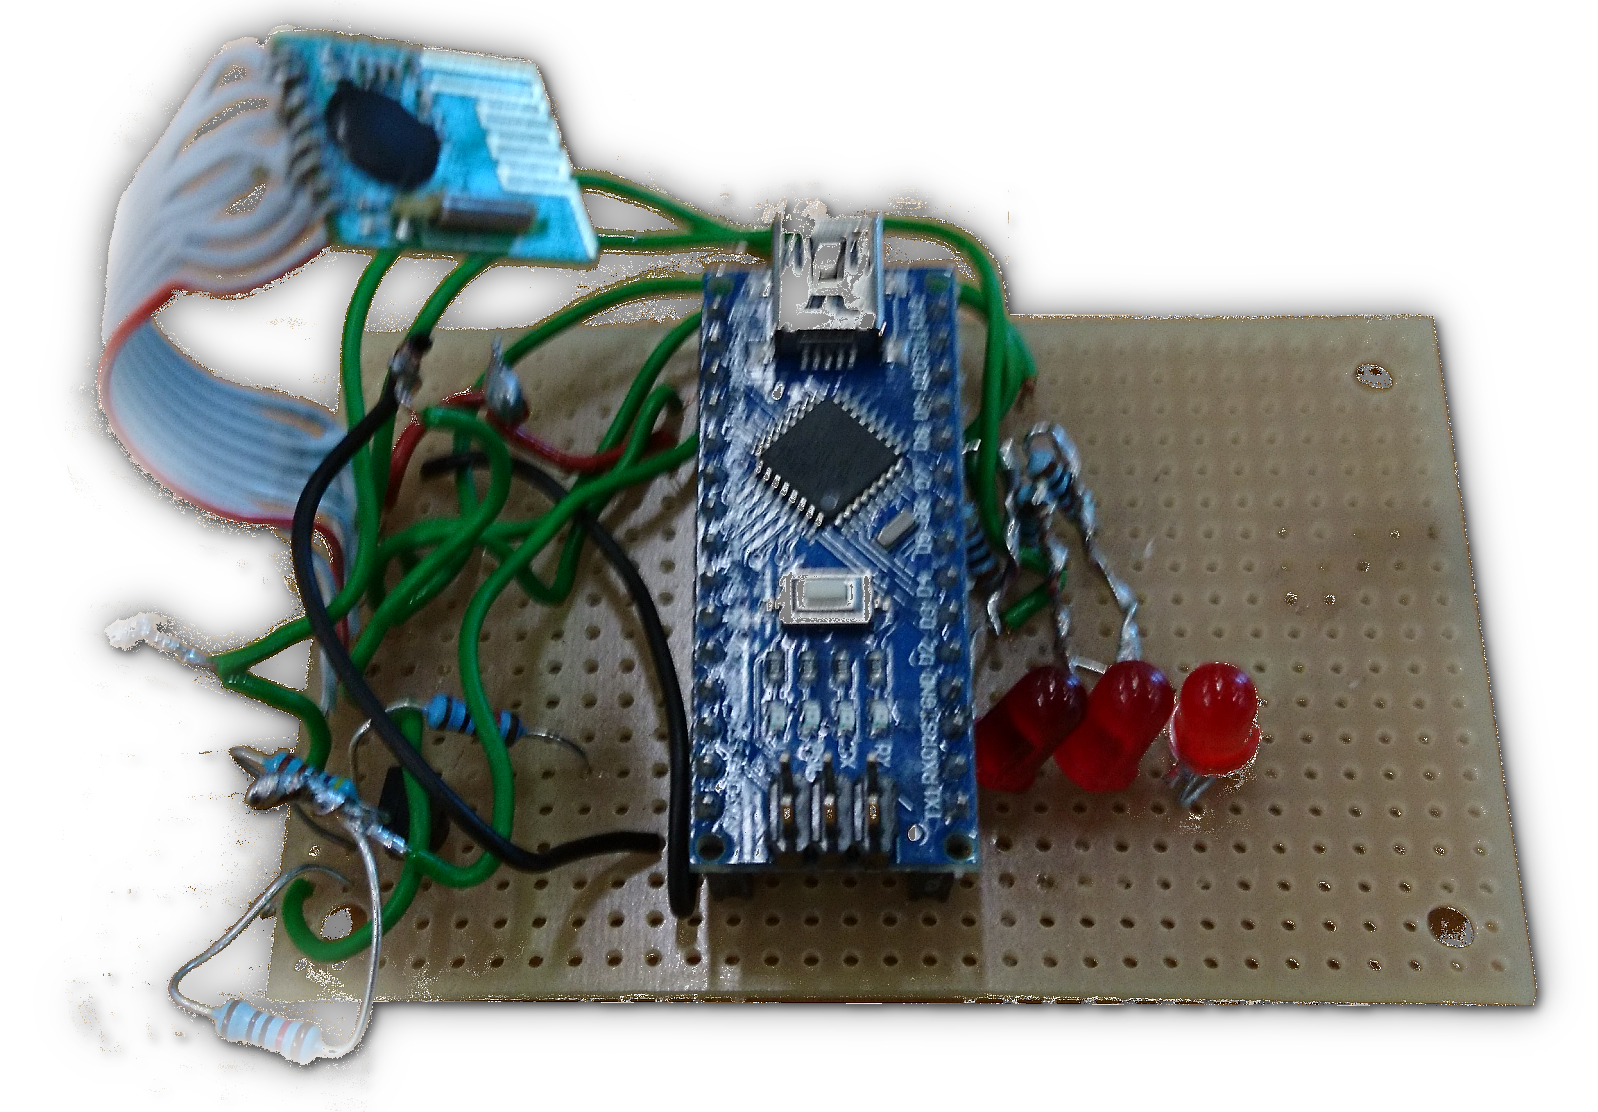
\includegraphics[scale=0.2]{images/receiver}
	\caption{Empfänger zur Validierung des Magic Glove}
	\label{fig:receiver}
\end{figure}

In diesem Kapitel finden sich folgende Validierungen:\\
Hardware
\begin{itemize}
	\item Validierung Batteriemanagement
	\item Aussteuerung Analogteil
\end{itemize}
Software
\begin{itemize}
	\item Validierung ADC-Wandler
	\item Übertragungsgeschwindigkeit RFM75
\end{itemize}

\subsection{Hardware}
\subsubsection*{Validierung Batteriemanagement}
Zum Testen der Ladeschaltung auf dem Magic Glove wird die verwendete Li-Ionen-Zelle mit einem Lastwiderstand auf 20\% entladen und dann eine Spannung von 5 Volt an den Schaltungsteil angelegt. Nach 6 Stunden wird die Spannung des Akkumulators gemessen. Zusammengefasst sind die Messungen in der Tabelle \ref{tab:MagicGlovevalid1}.
% befand sich die Akkumulatorenspannung auf 4.15 Volt.
	\begin{center}
	\begin{tabular}{l|c}
		\hline 
		Gemessene Akkuzelle (Entladen) & 3.72 V \\ \hline
		Gemessene Spannung nach 6h & 4.15V \\ \hline
	\end{tabular} 
	\captionof{table}{Messung Übertragungsgeschwindigkeit RFM75 Resultate}
	\label{tab:MagicGlovevalid1}
\end{center}

\subsubsection*{Aussteuerung Analogteil}
Um die Aussteuerung des Operationsverstärkers im Analogteil zu messen, wird einerseits mit dem Oszilloskop die Spannung am ADC-Eingang gemessen und andererseits der gemessene Wert via UART-Kommunikation an den Computer gesendet.
Die maximale Aussteuerung, die mit dem Operationsverstärker erreicht werden konnte, beträgt 3.03V. Dies entspricht einer Aussteuerung von 91.7\% am ADC-Eingang, falls dessen Referenz auf genau 3.3V ist. Zusammengefasst sind die Messungen in der Tabelle \ref{tab:MagicGlovevalid2}.
\begin{center}
	\begin{tabular}{l|c}
		\hline 
		Gemessene min. Spannung & 21.7mV \\ \hline
		Gemessene max. Spannung & 3.03V \\ \hline
	\end{tabular} 
	\captionof{table}{ADC-Messung Magic Glove}
	\label{tab:MagicGlovevalid2}
\end{center}

\subsection{Software}
\subsubsection*{Validierung ADC-Wandler}
Für die Validierung der Software wurde ein separater Empfänger mit einem Arduino Nano gebaut. Dieser kann über USB angesteuert werden und sendet die gemessenen Werte über UART an den angeschlossenen Computer.
Nach der Aussteuerung wird der Flex-Sensor an mehrere vordefinierte Positionen bewegt. Zusammengefasst sind die Messungen in der Tabelle \ref{tab:MagicGlovevalidADC}.
%er dazu parallel gemessene numerische Wert auf dem ADC-Eingang war 939. 
%Da die Werte anschliessend mit einem Faktor 0.25 verkleinert werden, kann der Flex-Sensor die Schaltung nahezu komplett aussteuern.
\begin{center}
	\begin{tabular}{l|c}
		\hline 
		Kleinster nummerischer ADC-Wert & 7 \\ \hline
		Höchster nummerischer ADC-Wert & 256 \\ \hline
	\end{tabular} 
	\captionof{table}{ADC-Messung Magic Glove}
	\label{tab:MagicGlovevalidADC}
\end{center}

\subsubsection*{Übertragungsgeschwindigkeit RFM75}
Für diesen Test wird auf dem Empfänger-PCB eine LED an- beziehungsweise ausgeschaltet. Dieser Puls wird dann wiederum mit dem Oszilloskop gemessen. Ist die daraus entstehende Höchstfrequenz höher als die gewünschte Übertragungsgeschwindigkeit, kann problemlos die erforderliche Datenmenge gesendet werden. Zusammengefasst ist dieser Test in der Tabelle \ref{tab:MagicGlovevalid3}.
\begin{center}
	\begin{tabular}{l|c}
		\hline 
		Gewünschte Sendefrequenz & 100 Samples/Sekunde \\ \hline
		Gemessene Zeit zwischen Paketen & 3.58ms \\ \hline
		Resultierende Empfangsfrequenz & ca. 279 Samples/Sekunde \\ \hline
	\end{tabular} 
	\captionof{table}{Messung Übertragungsgeschwindigkeit RFM75 Resultate}
	\label{tab:MagicGlovevalid3}
\end{center}
%%%%%%%%%%%%%%%%%%%%%%%%%%%%%%%%%%%%%%%%%%%%%%%%%%%%%%%%%%%%%%%%
% Stromversorgung
%%%%%%%%%%%%%%%%%%%%%%%%%%%%%%%%%%%%%%%%%%%%%%%%%%%%%%%%%%%%%%%%
\section{Stromversorgung} \label{ValidStromversorgung}

%%%%%%%%%%%%%%%%%%%%%%%%%%%%%%%%%%%%%%%%%%%%%%%%%%%%%%%%%%%%%%%%
% MC
Damit die Ergebnisse reproduzierbar sind, wird die Stromversorgung auf einem Prüfstand getestet. In der ersten Validierungsphase wird der Print und die Software ohne Akku getestet, welcher dann in der zweiten Validierungsphase angeschlossen wird. \textbf{Achtung:} Da es sich beim Akku um einen LiPo-Akku handelt, welcher einen Spitzenstrom von bis zu 500A liefert, soll der Print zuerst auf allfällige Kurzschlüsse geprüft werden.   
\\
In diesem Kapitel finden sich folgende Validierungen:\\
Hardware
\begin{itemize}
	\item Funktion der FETs
	\item Messung der Spannungen
	\item Ausmessung des High-Side-Driver
\end{itemize}
Software
\begin{itemize}
	\item Einlesen Spannung und Ströme
	\item PWM-Regelung
	\item Balancing Steuerung
\end{itemize}

\subsection{Hardware}
\subsubsection*{FETs}
Als erstes werden die FETs des Balancing der Reihe nach eingeschaltet. Dabei wird jeweils eine Spannung von 4.2V zwischen Zellanschluss 6 und 5, Zellanschluss 5 und 4 usw. angeschlossen. Sobald die richtige Spannung angeschlossen ist und derjenige FET durchgeschaltet ist, soll einen Strom von 100mA fliessen. In der Tabelle \ref{tab:StromBalancing} sind die Messungen zusammengefasst.

\begin{center}
	\begin{tabular}{l|c}
		Messobjekt & Strom \\ \hline
		Balance Zelle 1 & $103.1mA$ \\ \hline
		Balance Zelle 2 & $102.7mA$ \\ \hline
		Balance Zelle 3 & $103.5mA$ \\ \hline
		Balance Zelle 4 & $103.4mA$ \\ \hline
		Balance Zelle 5 & $102.9mA$ \\ \hline
		Balance Zelle 6 & $102.8mA$ \\ \hline
	\end{tabular} 
	\captionof{table}{Balancing Strom je Zelle}
	\label{tab:StromBalancing}
\end{center}

Weiter werden die FETs getestet, welche die Spannung zum Motorcontrollboard steuern. Dabei wird ein Leistungswiderstand auf Masse geschaltet. Das Ergebnis ist in der Tabelle \ref{tab:fetmessbedzumotorcontrol} ersichtlich.

\begin{center}
	\begin{tabular}{l|c}
		\hline 
		Versorgungsspannung & $25V$ \\ \hline
		Lastwiderstand & $2.5\Omega$ \\ \hline
	\end{tabular} 
	\captionof{table}{Messbedingungen FETs zu Motorcontroll}
	\label{tab:fetmessbedzumotorcontrol}
\end{center}

Nun soll ein Strom von rund 10A fliessen. Dabei sollen die FETs nur leicht bzw. gar nicht warm werden. Die Messbedingung ist in der Tabelle \ref{tab:StromMotorcontrollFET} festgehalten.

\begin{center}
	\begin{tabular}{l|c}
		\hline 
		Strom & $10.02A$ \\ \hline
	\end{tabular} 
	\captionof{table}{Strom durch Motorcontrol-FET}
	\label{tab:StromMotorcontrollFET}
\end{center}

Der FET wurde bei diesem Strom kaum merklich warm.

Der FET, welcher fürs Laden zuständig ist, wird bei der Ausmessung des High-Side-Driver getestet.

\subsubsection*{Spannungsmessung}
Nun werden die einzelnen Spannungsteiler ausgemessen. Dabei werden am Balancing-Anschluss jeweils die einzelnen Zellen angeschlossen. Weiter wird die Ladespannung angeschlossen. Nun soll an den Spannungsteiler gemessen werden. Der Akku soll voll geladen sein und die Spannungsteiler dürfen die Mikrocontroller-Speisung nicht überschreiten. Die Messbedingungen sind in der Tabelle \ref{tab:BedingungSpannungsmessungen} aufgelistet.

\begin{center}
	\begin{tabular}{l|c}
		\hline 
		Versorgungsspannung Batterieseitig & $25V$ \\ \hline
		Versorgungsspannung Ladeseitig & $30V$ \\ \hline
		Versorgungsspannung Mikrocontroller & $5V$ \\ \hline
		Versorgungsspannung High-Side-Driver & $15V$ \\ \hline
		
	\end{tabular} 
	\captionof{table}{Messbedingung Spannungsmessungen}
	\label{tab:BedingungSpannungsmessungen}
\end{center}

Um zu Prüfen, ob die Spannungsregelung funktioniert, wird auch diese gemessen. Die Messergebnisse finden sich in der Tabelle \ref{tab:Spannungsmessungen}.

\begin{center}
	\begin{tabular}{l|c|c}
		Messobjekt & Gemessene Spannung & Skalierungsfaktor \\ \hline
		Versorgungsspannung Mikrocontroller & $5.016V$ & - \\ \hline
		Versorgungsspannung High-Side-Driver & $15.65V$ & - \\ \hline
		Zelle 1 & $4.132V / 4.132V$ & 1 \\ \hline
		Zelle 2 & $8.268V / 4.077V$ & 0.493 \\ \hline
		Zelle 3 & $12.34V / 4.064V$ & 0.329 \\ \hline
		Zelle 4 & $16.45V / 4.096V$ & 0.249 \\ \hline
		Zelle 5 & $20.85V / 4.153V$ & 0.202 \\ \hline
		Zelle 6 & $24.72V / 4.120V$ & 0.162 \\ \hline
		Spannungsteiler Ladeseitig & $30.01V / 2.132V$ & 0.071\\ \hline
	\end{tabular} 
	\captionof{table}{Gemessene Spannung}
	\label{tab:Spannungsmessungen}
\end{center}

Die Skalierungsfaktoren lagen ziemlich genau an unserem gewünschten Ergebnis. Somit konnten die berechneten Werte für die Widerstände übernommen werden.  

\subsubsection*{High-Side-Driver}
\label{Highside-Driver}
Damit der High-Side-Driver getestet werden kann, soll die Batterie entfernt und einen Leistungswiderstand von rund 5$\Omega$ angeschlossen werden. Der High-Side-Driver wird dabei extern mit 15V gespeist. Als erstes wird am Mikrocontroller ein PWM-Signal mit 50\% Duty-Cycle ausgegeben. Dabei soll am Ausgang des High-Side-Driver dasselbe Signal mit 15V Spannungsspitze anliegen. Nun wird eine externe Ladespannung angeschlossen. Diese liegt für Testzwecke bei 15V. Dabei soll die Strombegrenzung auf 3A eingestellt sein. Nun wird der Duty-Cycle ständig erhöht. Dabei wird der Strom beim Leistungswiderstand gemessen und mit nachfolgender Tabelle \ref{tab:LadestromHighsideDriver} abgeglichen.

\begin{center}
	\begin{tabular}{l|c}
		\hline 
		Duty-Cycle: 0\% & $0A$ \\ \hline
		Duty-Cycle: 20\% & $0.6A$ \\ \hline
		Duty-Cycle: 40\% & $1.2A$ \\ \hline
		Duty-Cycle: 60\% & $1.8A$ \\ \hline
		Duty-Cycle: 80\% & $2.4A$ \\ \hline
	\end{tabular} 
	\captionof{table}{Ladestrom bei verschiedenen Duty-Cycle}
	\label{tab:LadestromHighsideDriver}
\end{center}

Einen Duty-Cycle von 100\% wird nicht geprüft, da der High-Side-Driver nicht dazu ausgelegt ist, einen FET dauerhaft durch zusteuern.

Dies konnte aufgrund eines defekten High-Side-Drivers nicht evaluiert werden. 

\subsection{Software}
Um diese Ergebnisse zu überprüfen, muss am UART des Mikrocontroller ein TTL-Kabel angeschlossen werden.

\subsubsection*{ADC}
Um die einzelnen Zellen auszulesen, kann die Batterie sowie eine Ladespannung von mindestens 30V angeschlossen werden. Dabei werden die einzelnen Spannungen jede Sekunde einmal über den UART Port ausgegeben. Dabei soll die Spannung mit dem Multimeter gemessen und überprüft werden. Um den Strom zu messen, wird die Messung gleich wie in Kapitel \ref{Highside-Driver} aufgebaut. Die gemessenen Spannungen sind in der Tabelle \ref{tab:Spannungengemessen} aufgeführt.

\begin{center}
	\begin{tabular}{l|c|c|c}
		ADC-Eingang & Spannung Multimeter & Spannung ADC & Differenz \\ \hline
		Zelle 1 & $4.132V$ & $4.116V$ & $0.016V$ \\ \hline
		Zelle 2 & $4.134V$ & $4.121V$ & $0.013V$ \\ \hline
		Zelle 3 & $4.065V$ & $4.028V$ & $0.037V$ \\ \hline
		Zelle 4 & $4.117V$ & $4.106V$ & $0.011V$ \\ \hline
		Zelle 5 & $4.132V$ & $4.131V$ & $0.001V$ \\ \hline
		Zelle 6 & $4.131V$ & $4.111V$ & $0.020V$ \\ \hline
		Ladespannung & $2.113V$ & $2.105V$ & $0.008$ \\ \hline
	\end{tabular} 
	\captionof{table}{gemessene Spannungen}
	\label{tab:Spannungengemessen}
\end{center}

All diese Werte liegen innerhalb der Toleranz des ADCs des Mikrocontrollers und sind somit ausreichend genau.

\subsubsection*{PWM-Regelung}
Um das PWM-Signal zu überprüfen, wird Softwareseitig ein vordefinierter Strom eingestellt. Dabei wird anstatt des Akkus ein veränderbarer Leistungswiderstand am Ausgang angeschlossen. Nun wird der Widerstand verändert und überprüft, ob die Software richtig nachregelt. Die Vorgabe für des PWM-Signals ist in der Tabelle \ref{tab:LadestromPWM} festgehalten. Das Ergebnis ist in der Abbildung \ref{fig:PWM_uC} grafisch dargestellt.
\begin{center}
	\begin{tabular}{l|c}
		\hline 
		Teststrom & $1A$ \\ \hline
		${f}_{PWM}$ & $32kH$ \\ \hline
	\end{tabular} 
	\captionof{table}{Vorgabe PWM}
	\label{tab:LadestromPWM}
\end{center}

\begin{figure} [H]
	\centering
	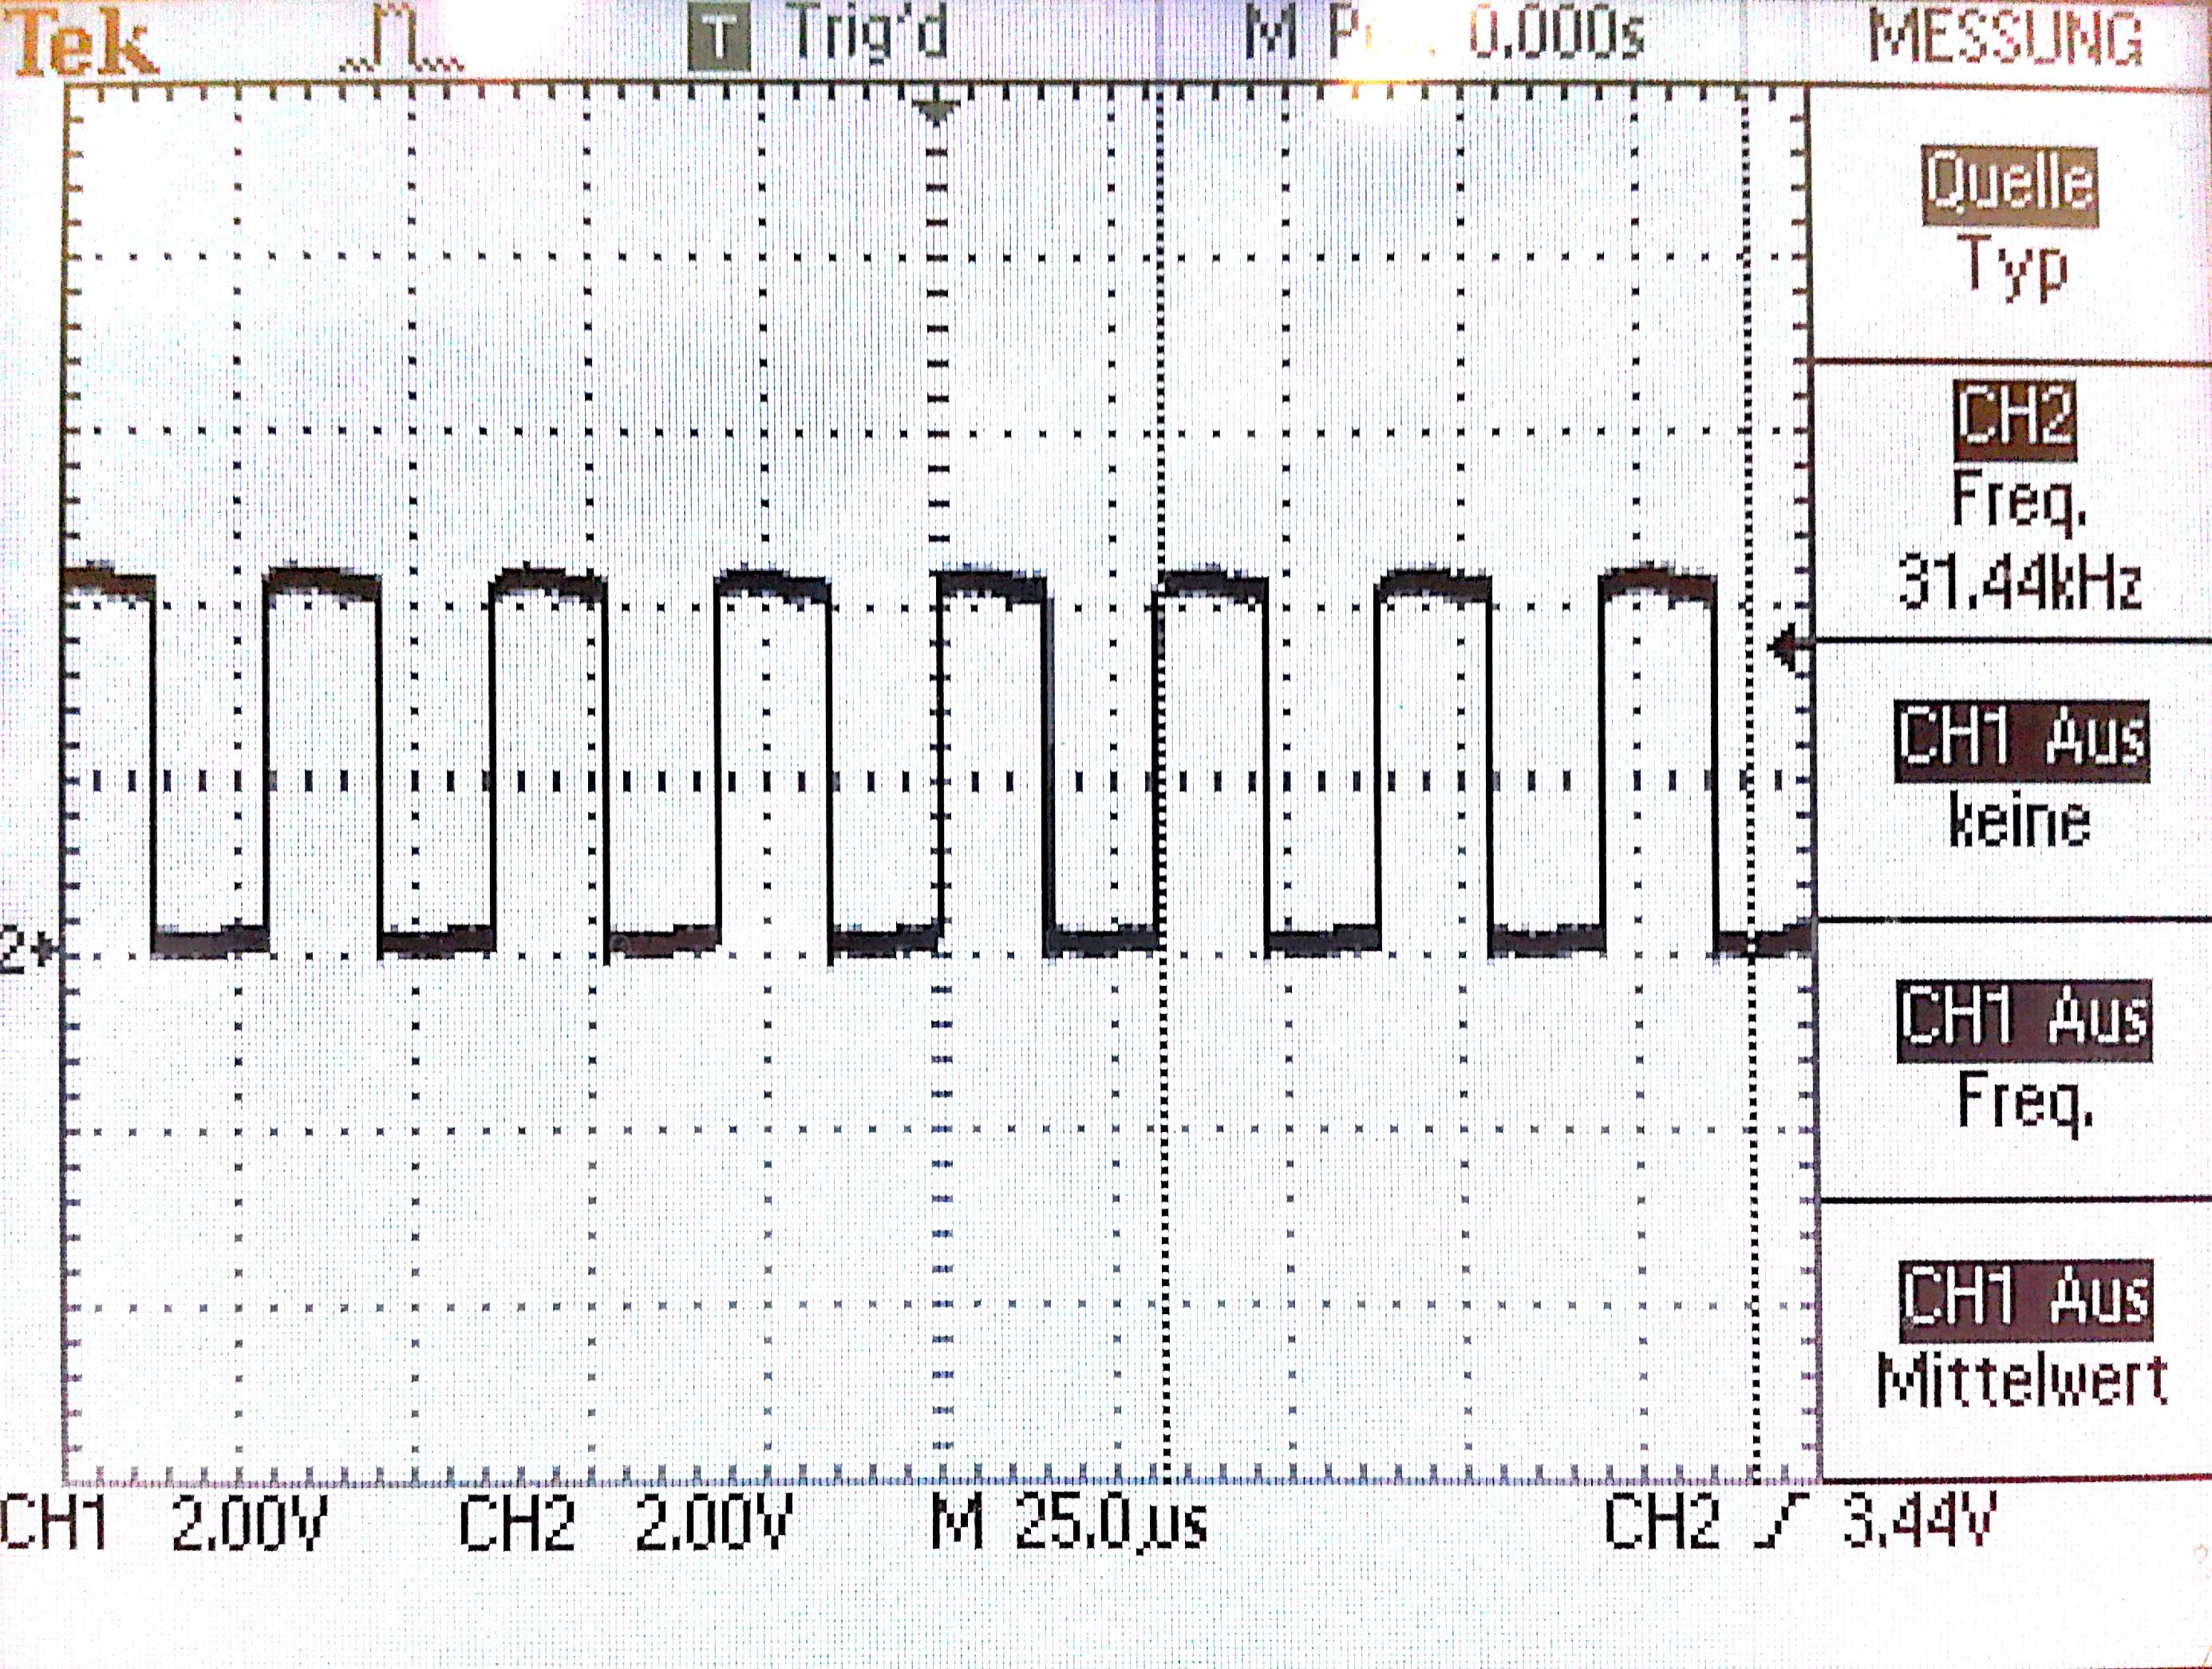
\includegraphics[width=0.5\linewidth]{images/PWM.jpg}
	\caption{PWM Mikrocontroller bei 50\% Duty-Cycle}
	\label{fig:PWM_uC}
\end{figure}

\subsubsection{Balancing-Regelung}
Für diese Validierung wird jeweils eine Spannung an den Zellen-Anschlüssen angeschlossen. Dabei wird überprüft, ob die Software bei den jeweiligen Zellen die FETs durchsteuert, um  die gleiche Spannung wie bei den anderen Zellen zu erreichen.
%Resultate??

%\begin{itemize}
%\item Einlesen Spannung und Ströme
%\item PWM-Regelung
%\item Balancing Steuerung
%\end{itemize}

%%%%%%%%%%%%%%%%%%%%%%%%%%%%%%%%%%%%%%%%%%%%%%%%%%%%%%%%%%%%%%%%
\section{Motoransteuerung} \label{ValidMotoransteuerung}
Um reproduzierbare Ergebnisse zu erzielen, wird die Motoransteuerung auf einem Prüfstand getestet. Dazu wird der Motor ohne Last befestigt und die Schaltung von einem Netzteil gespeist. Weiter wird die Motoransteuerung in einzelnen Blöcken validiert. Dabei wird unterschieden in Hardware und Software.\\
\\
Hardware
\begin{itemize}
	\item Funktion der FETs
	\item Spannungsmessung mit Spannungsteiler
\end{itemize}
Software
\begin{itemize}
	\item Einlesen der Spannungen und Ströme
	\item SVPWM (Raumvektormodulation)
	\item Positions- und Geschwindigkeitsbeobachter
	\item D und Q Stromregler
\end{itemize}

\subsection{Hardware}
\subsubsection*{FETs}
Die FETs werden der Reihe nach von der Software eingeschaltet. Zum Test der FETs wird am Ausgang ein Lastwiderstand auf Masse geschaltet. So kann die Spannung am Ausgang gemessen und aufgezeichnet werden. Zusätzlich wird die Gatespannung gemessen. In der Tabelle \ref{tab:fetmessbed} sind die Messbedingungen ersichtlich.

\begin{center}
	\begin{tabular}{l|c}
		\hline 
		Versorgungsspannung & $15V$ \\ \hline
		Lastwiderstand & $1k\Omega$ \\ \hline
		Gatestrom Treiber & $1.7A$ \\ \hline
	\end{tabular} 
	\captionof{table}{Messbedingungen FETs}
	\label{tab:fetmessbed}
\end{center}

Zur Gunsten der Übersichtlichkeit wird nur die Messung eines FETs (Abb. \ref{fig:hsfet})dargestellt, die zugehörigen Einstellungen sind in der Tabelle \ref{tab:MotorFET_Scopeeinstellung} aufgeführt.

\begin{figure} [H]
	\centering
	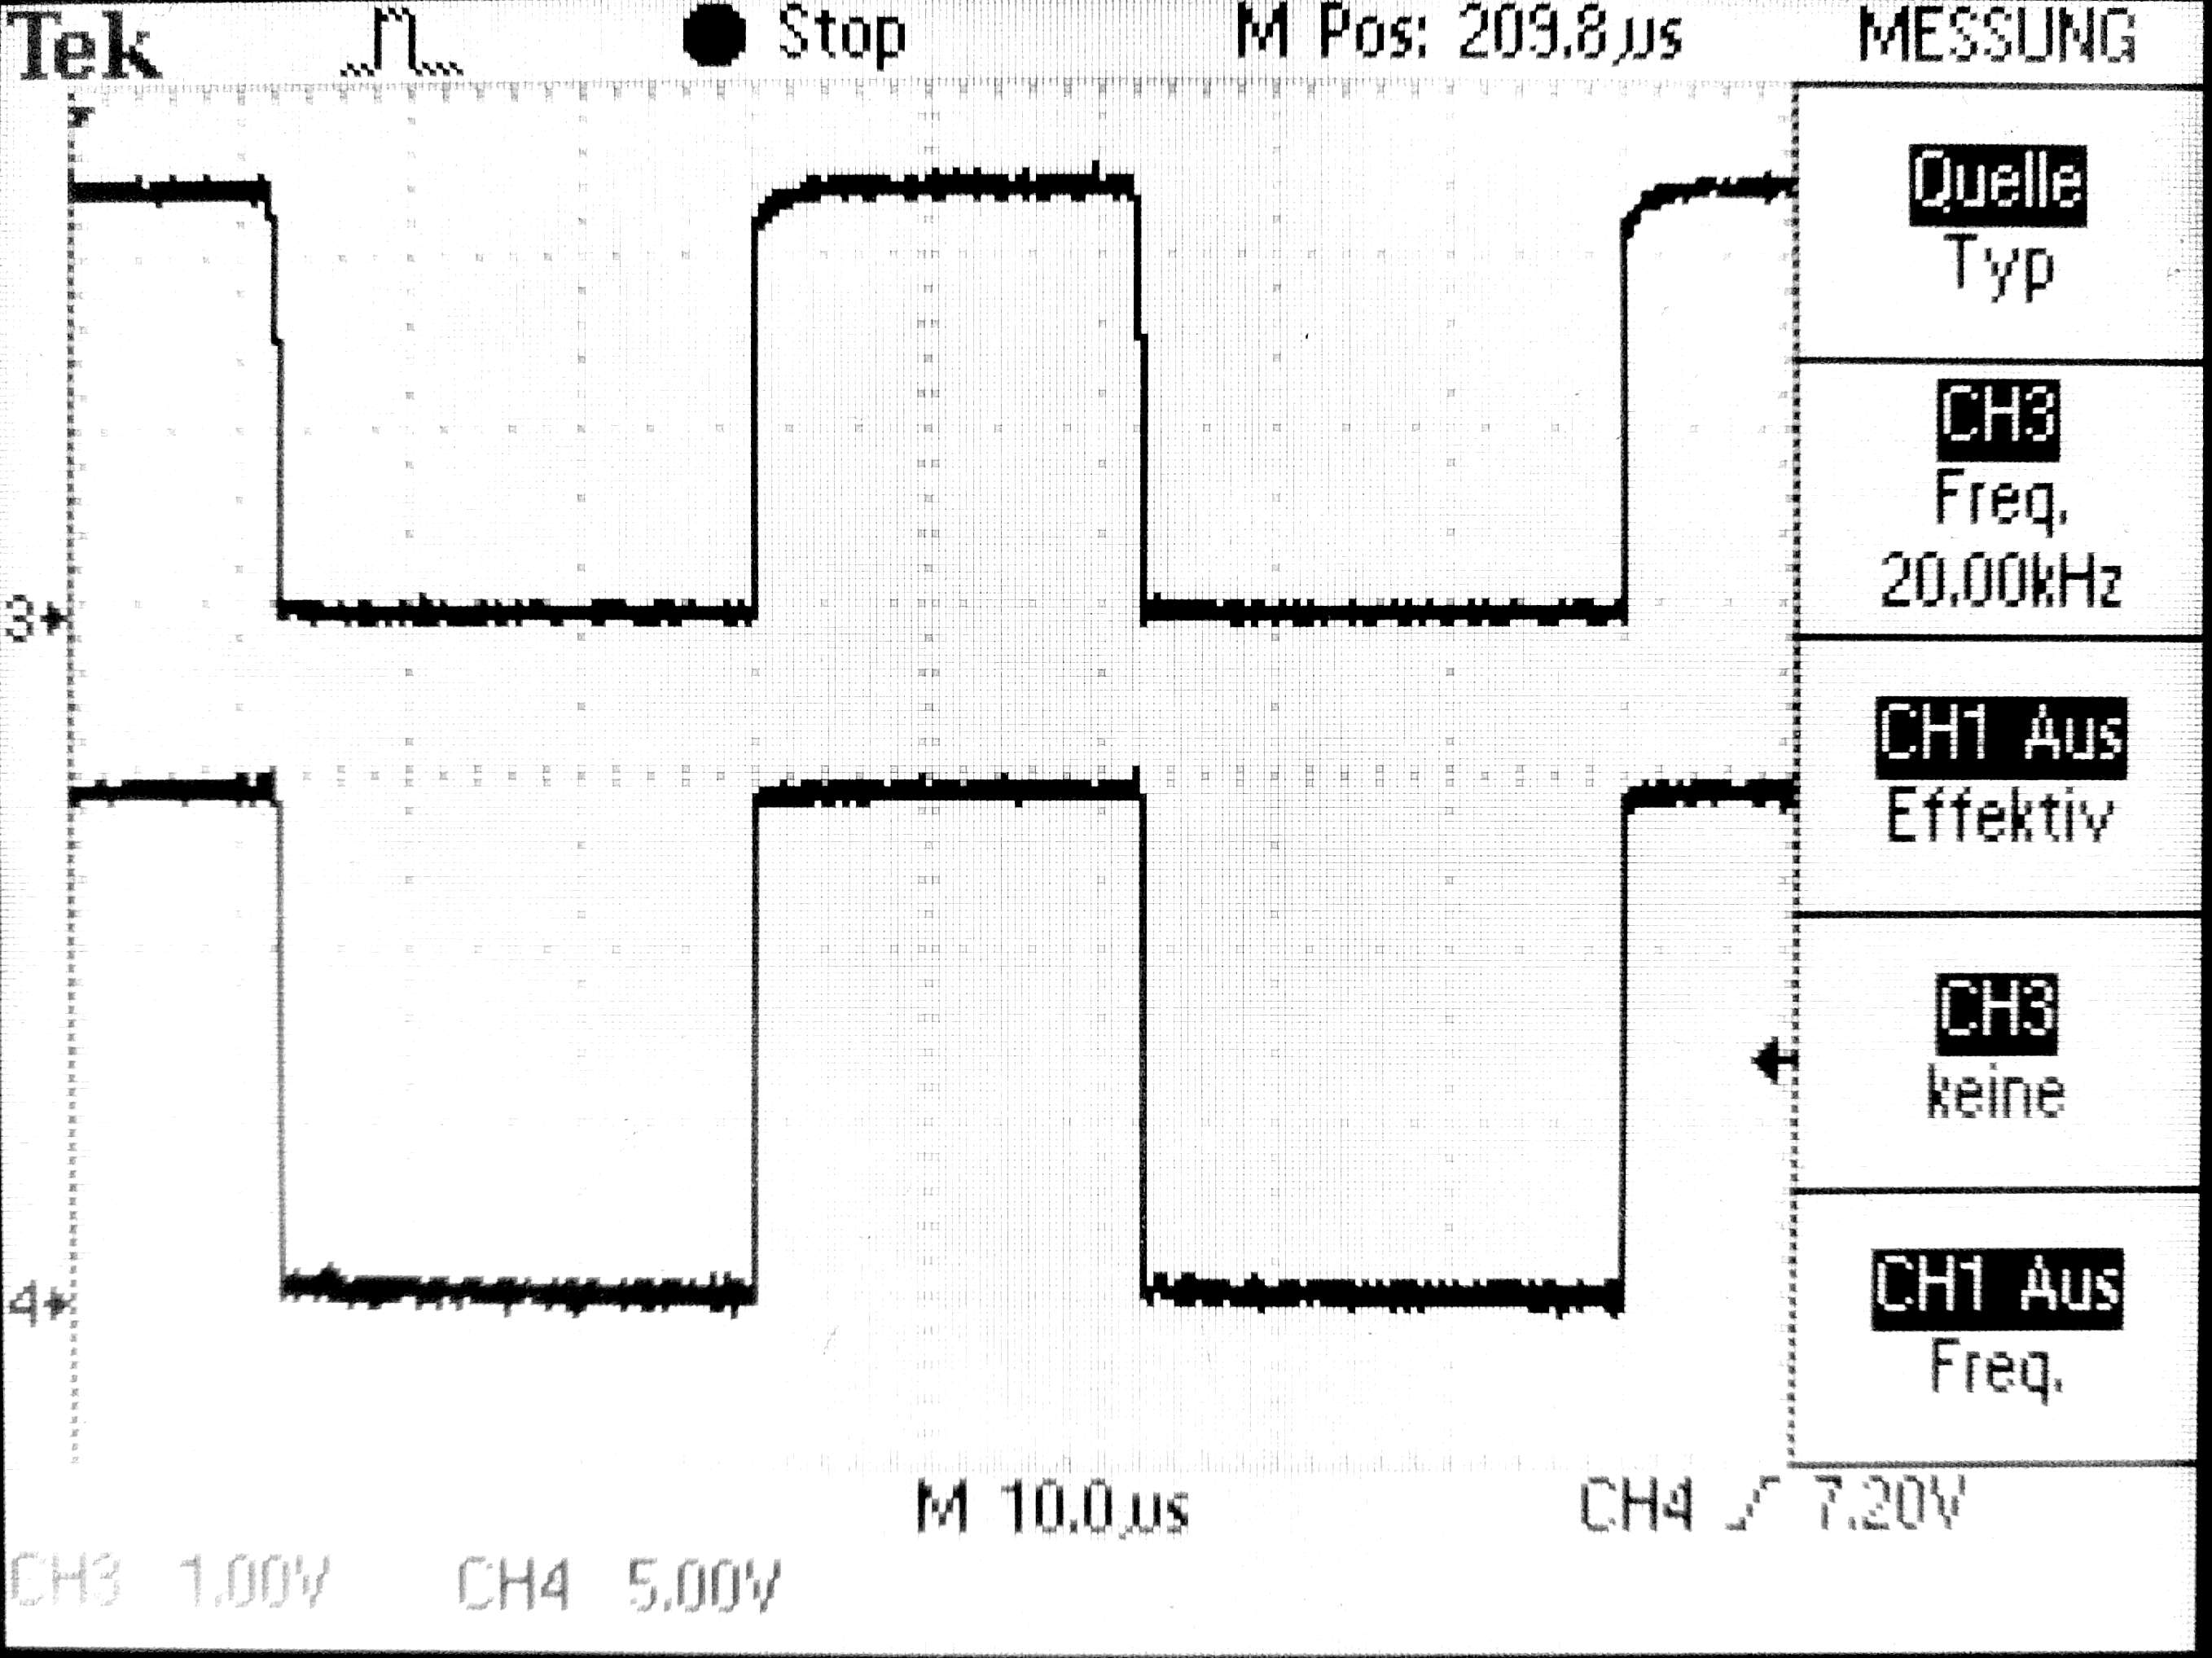
\includegraphics[width=0.6\linewidth]{images/valmcfet.jpg}
	\caption{Einschalten High-Side-FET}
	\label{fig:hsfet}
\end{figure}

\begin{center}
	\begin{tabular}{l|l|l}
		\hline 
		Kanal 1 & High FET A Gate & Mit 10x Abschwächung\\ \hline
		Kanal 2 & Spannung Phase A & {}\\ \hline
	\end{tabular}
	\captionof{table}{Scopeeinstellungen}
	\label{tab:MotorFET_Scopeeinstellung}
\end{center}

Der Kanal 1 zeigt die Steuerspannung am Gate des FETs. Sie wird vom Treiber IC erzeugt und beträgt im eingeschalteten Zustand 24V, das sind rund 7V Gate-Source-Spannung. Dies sichert ein schnelles Durchschalten des FETs. Erkennbar ist dies an der steilen Flanke am Ausgang der Halbbrücke, zu sehen auf Kanal 4.

\subsubsection*{Spannungsmessung}
Ist der Mikrocontroller im Resetzustand, sind alle FETs ausgeschaltet. So kann eine Spannung an die Ausgänge der Halbbrücke gegeben und am Ausgang der Spannungsteiler die Spannung gemessen werden. Diese darf bei einem bestimmten Eingangsspannungsbereich die Mikrocontroller-Speisung nicht überschreiten. Die Messbedingungen sind in der Tabelle \ref{tab:vmessbed}, die Ergebnisse in der Tabelle \ref{tab:spannteiler} zusammengefasst.

\begin{center}
	\begin{tabular}{l|c}
		\hline 
		Versorgungsspannungsbereich & $0$ bis $20V$ \\ \hline
		Mikrocontroller-Speisung & $3.3V$ \\ \hline
		Spannungsteiler Faktor & $0.0534$ \\ \hline
	\end{tabular} 
	\captionof{table}{Messbedingungen Spannungsmessung}
	\label{tab:vmessbed}
\end{center}

\begin{center}
	\begin{tabular}{l|l|l}
		Spannung an Phase & Spannung gemessen am Mikrocontroller & Faktor\\ \hline
		5V & 0.268V & 0.0536\\ \hline
		10V & 0.536V & 0.0536\\ \hline
		15V & 0.804V & 0.0536\\ \hline
		20V & 1.072V & 0.0536\\ \hline
	\end{tabular} 
	\captionof{table}{Spannungsmessung Spannungsteiler}
	\label{tab:spannteiler}
\end{center}

Die Spannungen, gemessen nach den Spannungsteiler, entsprechen exakt dem angelegten Wert mal dem Teilungsfaktor. Dies ist erstaunlich exakt und völlig innerhalb der Widerstandstoleranzen.

\subsection{Software}
\subsubsection*{Einlesen der Spannungen}
Über die Shell des Mikrocontrollers werden alle gemessenen Spannungen periodisch ausgegeben. Um die Spannungen zu messen, werden die FETs ausgeschaltet und eine Spannung an den Ausgängen angelegt. Um die Strommessung zu validieren, werden die Low-Side-FETs eingeschaltet und ein Strom an den Ausgängen eingespeist. So kann der gesamte Signalpfad der Messungen validiert werden. Die Messparameter sind in der Tabelle \ref{tab:swvmessbed} zusammengefasst, die Ergebnisse finden sich in der Tabelle \ref{tab:spannsw} und \ref{tab:stromsw}.

\begin{center}
	\begin{tabular}{l|c}
		\hline 
		Testspannung & $0$ bis $20V$ \\ \hline
		Teststrom & $0$ bis $2A$ \\ \hline
	\end{tabular} 
	\captionof{table}{Messbedingungen Spannungsmessung Software}
	\label{tab:swvmessbed}
\end{center}

\begin{center}
	\begin{tabular}{l|l} 
		Spannung an Phase & Spannung gemessen vom Mikrocontroller \\ \hline
		5V & 3.7V\\ \hline
		10V & 8.5V\\ \hline
		15V & 13.3V\\ \hline
		20V & 18.0V\\ \hline
	\end{tabular} 
	\captionof{table}{Spannungsmessung Software}
	\label{tab:spannsw}
\end{center}

Die Spannungswerte weichen stark von den Sollwerten ab. Dies ist aber nicht weiter tragisch, da viel mehr der Spannungsunterschied von Bedeutung ist. Zudem wird beim FOC Verfahren nur die Versorgungsspannung gemessen.

\begin{center}
	\begin{tabular}{l|l}
		Strom & Gemessen vom Mikrocontroller \\ \hline
		0.5A & 0.587A\\ \hline
		1A & 1.007A\\ \hline
		1.5A & 1.511A\\ \hline
		2A & 1.930A\\ \hline
	\end{tabular} 
	\captionof{table}{Strommessung Software}
	\label{tab:stromsw}
\end{center}

Auch bei den Stromwerten ist der relative Unterschied wichtiger als der Absolutwert.

\subsubsection*{SVPWM Raumvektormodulation}
Für diese Validierung wird eine sinusförmige Spannung mit konstanter Frequenz und Amplitude berechnet und der SVPWM-Routine übergeben. Die Ein- und Ausgabedaten werden für eine Zeitdauer aufgezeichnet und dann an den Computer übertragen, wo sie dargestellt werden.

\begin{figure} [H]
	\centering
	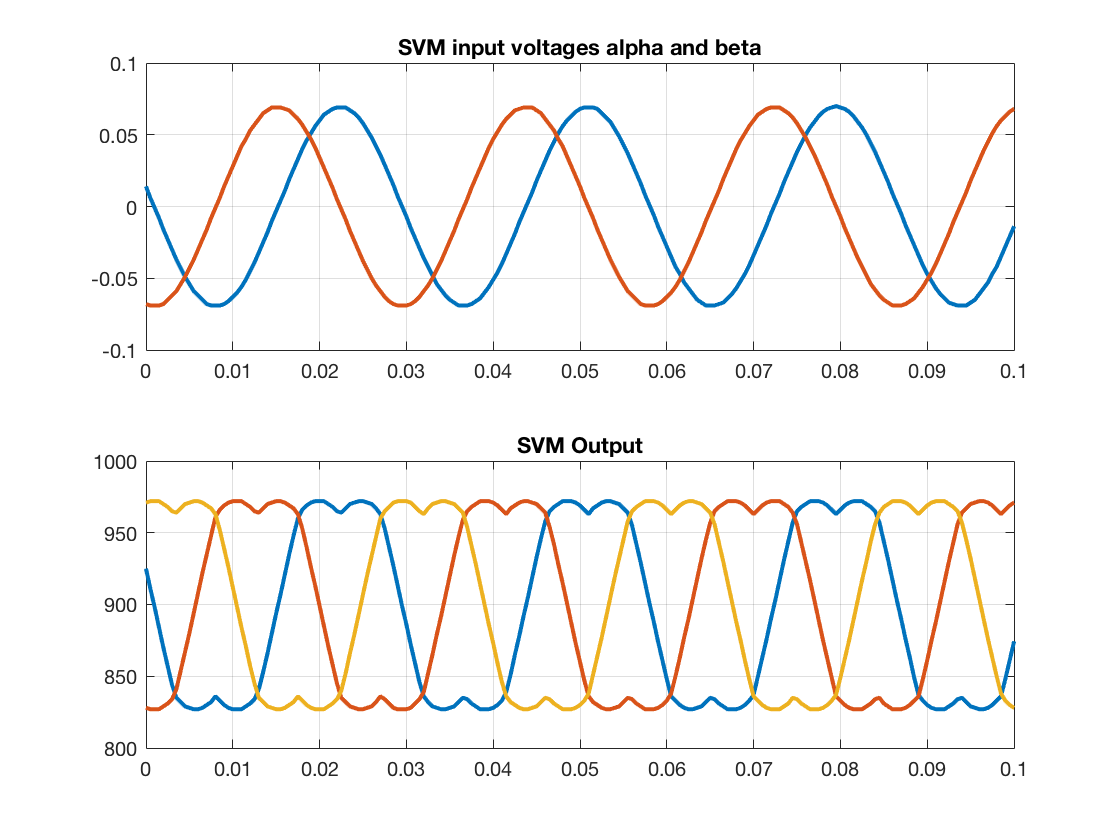
\includegraphics[width=0.8\linewidth]{images/valmcsvm.png}
	\caption{Validierung SVPWM Raumvektormodulation}
	\label{fig:svpwm}
\end{figure}

Im unteren Plot der Abbildung \ref{fig:svpwm} ist sehr gut der dreiphasige Sinus mit dritter harmonischer Welle zu sehen. Diese Werte entsprechen den Duty-Cycle der MOSFETs.

\subsubsection*{Positions- und Geschwindigkeitsbeobachter} \label{val:obs}
Nun wird der Motor zwangskommutiert. Das heisst, dass wieder eine sinusförmige Spannung mit konstanter Frequenz und Amplitude berechnet und auf die Halbbrücke geführt wird. Der Motor dreht nun mit einer konstanter Drehzahl. Die Ausgangswerte der Positions- und Geschwindigkeitsbeobachter werden erneut aufgezeichnet und mit dem Computer ausgewertet. In der Tabelle \ref{tab:obsmessbed} sind die Messbedingungen aufgelistet.

\begin{center}
	\begin{tabular}{l|c}
		\hline 
		$v_{d,set}$ & $0.0$ \\ \hline
		$v_{q,set}$ & $0.07$ \\ \hline
		$f_{set}$ & $35.0Hz$ \\ \hline
		Versorgungsspannung & $15V$ \\ \hline
	\end{tabular} 
	\captionof{table}{Messbedingungen Spannungsmessung Software}
	\label{tab:obsmessbed}
\end{center}

\begin{figure} [H]
	\centering
	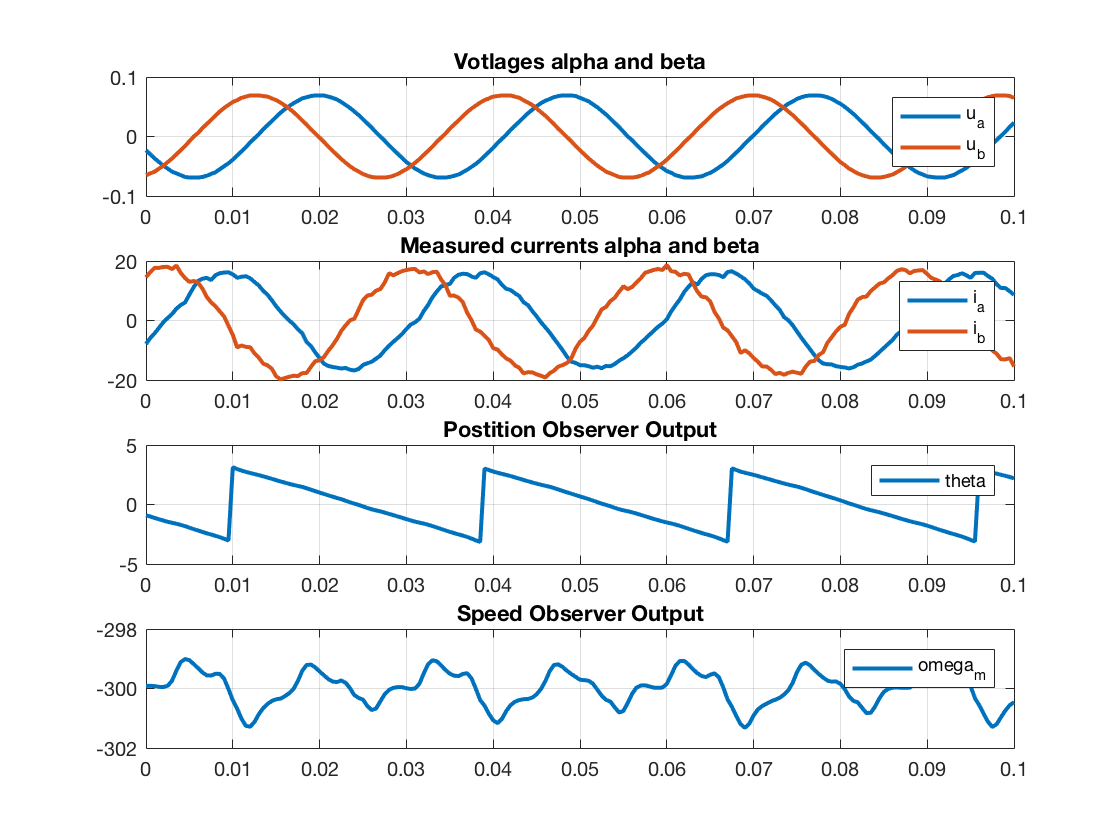
\includegraphics[width=0.8\linewidth]{images/valmcobserver.png}
	\caption{Validierung Positions- und Geschwindigkeitsbeobachter}
	\label{fig:observer}
\end{figure}

Abbildung \ref{fig:observer} zeigt in den ersten beiden Plots die Eingabewerte des Positionsbeobachters. Die gemessenen Ströme sind ungefiltert dargestellt und nur von kleinem Rauschen behaftet. Die Positionsschätzung theta hat ebenfalls nur einen kleinen Rippel und kann gut für die benötigten Transformationen verwendet werden.
Was in diesem Versuch nicht validiert werden kann, ist der Phasenversatz zwischen wahrem und geschätztem Winkel. Dazu wären unter Anderem ein Drehgeber am Motor und eine Datenauswertung nötig, welche zeitkritisch die berechneten und gemessenen Grössen aufzeichnen kann.

Die Schätzung der Drehzahl schwingt um den Mittelwert von 300rpm, was gemäss Formel \ref{eqt:omegaM-berechung} genau dem eingestellten Wert entspricht:

\begin{equation}
	\omega_m [rpm] = \frac{60 \cdot \omega_e}{p} = \frac{60 \cdot 35Hz}{7} = 300rpm
	\label{eqt:omegaM-berechung}
\end{equation}

Die Welligkeit wird vor dem Verwendung für den Stromregler mit einem Tiefpass gefiltert.

\subsubsection*{D und Q Stromregler}
Der letzte Validierungsschritt für die Motorsteuerung auf dem Prüfstand ist die Überprüfung der D und Q Stromregler. Wie bei Validierungsschritt \ref{val:obs} werden die Daten der Regler auf dem Mikrocontroller zwischengespeichert und anschliessend auf dem Computer dargestellt. Bei dieser Validierung wird der Motor im Closed-Loop-Modus betrieben. Es wird softwaremässig ein Sollwertsprung ausgeführt. Die Messbedingungen sind in der Tabelle \ref{tab:regmessbed} dargestellt.

\begin{center}
	\begin{tabular}{l|c}
		\hline 
		$i_{d,set}$ & $0$ \\ \hline
		$i_{q,set}$ & 3 auf 5 \\ \hline
		Versorgungsspannung & $21V$ \\ \hline
	\end{tabular} 
	\captionof{table}{Messbedingungen D und Q Stromregler}
	\label{tab:regmessbed}
\end{center}

\begin{figure} [H]
	\centering
	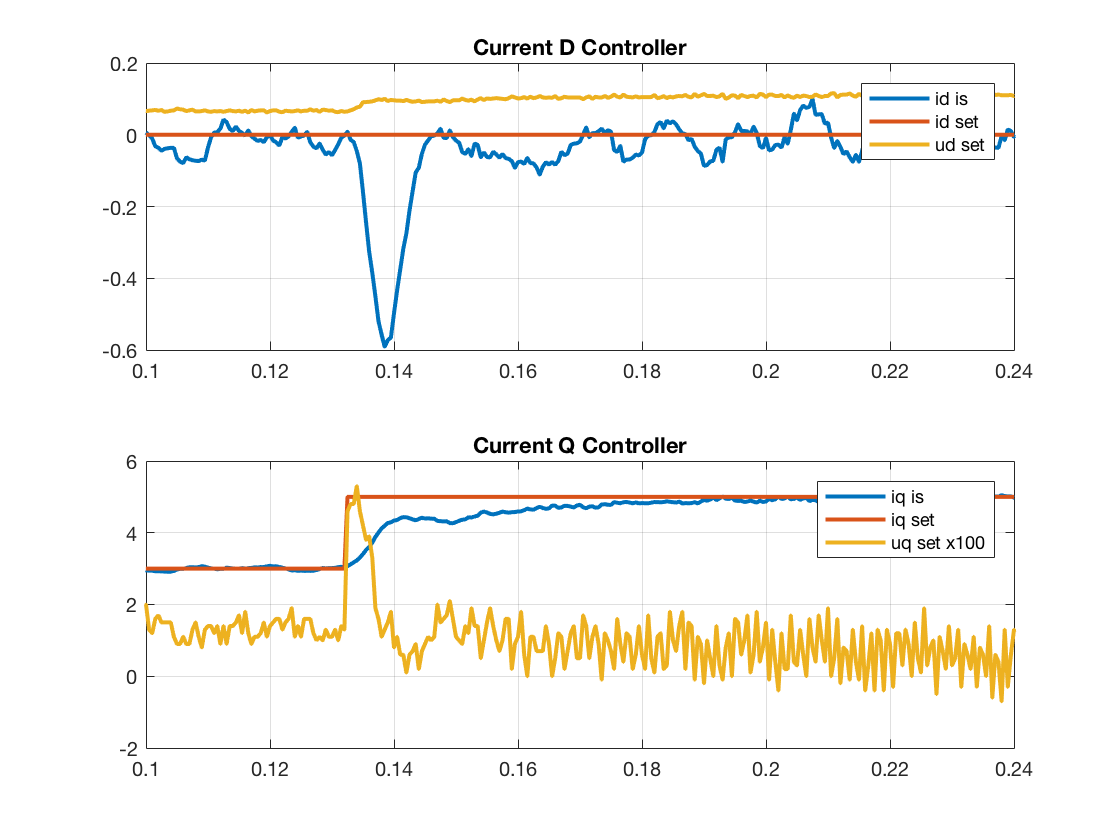
\includegraphics[width=0.8\linewidth]{images/valmccontrollers.png}
	\caption{Validierung D und Q Stromregler}
	\label{fig:reg}
\end{figure}

Abbildung \ref{fig:reg} zeigt die Sprungantwort der beiden Stromregler. Beide sind nicht perfekt und könnten noch optimiert werden. Da der Motor jedoch bei hohen Drehzahlen noch nicht dreht, wurde auf eine ausführliche Optimierung verzichtet. Was jedoch bestätigt werden kann ist, dass der Regler eine schnelle Sprungantwort hat und dank dem I-Anteil keine bleibende Regelabweichung vorhanden ist.


\subsubsection*{Fazit}
Die meisten Komponenten der Motorsteuerung funktionieren. Der Motor dreht jedoch nur bei langsamen Drehzahlen (kleiner 1000rpm) und mit wenig Drehmoment. Der Fehler liegt in der Implementierung des Stromreglers. Vermutlich ist es eine Sache der richtigen Parameter. Da das Umsetzen sehr zeitaufwändig ist, wurde darauf verzichtet.


%%%%%%%%%%%%%%%%%%%%%%%%%%%%%%%%%%%%%%%%%%%%%%%%%%%%%%%%%%%%%%%%
% Gesamtvalidierung
%%%%%%%%%%%%%%%%%%%%%%%%%%%%%%%%%%%%%%%%%%%%%%%%%%%%%%%%%%%%%%%%
\section{Gesamtvalidierung} \label{ValidGesamtv}
Nach eingehendem Testen der einzelnen Komponenten wird das Gesamtprodukt getestet. Dabei wird primär die Lauffähigkeit des Longboards und die Zusammenarbeit der einzelnen Komponenten untereinander untersucht. Insbesondere werden die im Pflichtenheft festgelegten Kriterien überprüft.

\begin{center}
	\begin{tabular}{p{0.5\textwidth}|p{0.5\textwidth}}
		Funktioniert und validiert & Nicht funktionsfähig \\ \hline 
		\begin{itemize}
			\item Stereung Magic Glove
			\item Stromversorgung: Verbindung zur Motoransteuerung
			\item Stromversorgung: Hardware
			\item Motoransteuerung: Hardware, Positionsbeobachter, SVPWM
		\end{itemize}
		&
		\begin{itemize}
			\item Stromversorgung: Laderegelung und Balancing
			\item Motoransteuerung: Motorregelung
		\end{itemize}
		\\ \hline
	\end{tabular} 
	\captionof{table}{Zusammenfassung der funktionierenden Komponenten}
	\label{tab:sumblk}
\end{center}

Tabelle \ref{tab:sumblk} fasst zusammen, welche Komponenten funktionieren und welche nicht. Die Steuerung mittels Magic Glove ist voll funktionsfähig und getestet. Um die Stromversorgung fertigzustellen, muss die Regelung des Ladevorgangs in der Software implementiert werden, sowie das Balancing. %Satz nid fertig...  verbessert werden
Die Hardware funktioniert und wurde validiert. Dasselbe ist der Fall bei der Motoransteuerung: Die Hardware wurde validiert und funktioniert einwandfrei. Das Einlesen der Ströme sowie das Schätzen der Rotorposition wurde ebenfalls validiert. Der Algorithmus zur Regelung des Motors ist auch implementiert, doch war keine Zeit mehr vorhanden für das Einstellen der Parameter. Der Motor dreht langsam und mit viel Drehmoment, doch bei hohen Drehzahlen blockiert er.

\subsubsection*{Alltagstauglichkeit} \label{ValidAlltag}
Wie bereits angedeutet, soll das fertige Board anhand von Testpersonen unterschiedlicher Skate-Erfahrung getestet werden. Die sanfte Anfahrmöglichkeit, die Manövrierfähigkeit und das allgemeine Wohlbefinden des Skaters sind die entscheidenden Kriterien. 
Testpersonen werden zufällig ausgewählt und die Bewertungen erfolgen nach subjektiver Einschätzung. 
Da das Longboard nicht fahrtüchtig ist, kann die Alltagstauglichkeit nicht getestet werden.

